\documentclass[12pt,a4paper]{article}
\pagestyle{plain}
\usepackage{fullpage}
\usepackage[english]{babel}
\usepackage{enumerate}

%equations
\usepackage[fleqn]{amsmath}
\numberwithin{equation}{section}

%figures
\usepackage[dvips]{graphicx}
\graphicspath{{./images/}}
\numberwithin{figure}{section}

%excercises
\newcounter{Exercise}
\setcounter{Exercise}{1}
\usepackage[dvipsnames]{xcolor}
\usepackage{framed}
\definecolor{shadecolor}{gray}{0.9}
\usepackage{caption}

%tables
\numberwithin{table}{section}

%specials
\usepackage{textcomp} %special (greek) characters as text
%\usepackage{pstricks} %
%\usepackage{ifthen} %
%\usepackage{calc} %
%\usepackage{isotope}
\usepackage{hyperref}
\usepackage[bottom]{footmisc} %footnote below figure
\usepackage{footnpag}%number footnotes per page


%document details
\author{N.G. Schultheiss \\ translated and adapted by K. Schadenberg}
\date{}
\title{Radio Telescopes}


\begin{document}
\maketitle

\section{Introduction}
In the previous module `The Expanding Universe' we saw that the universe is becoming ever larger. Light coming from the edges of the universe has undergone a large red shift. This shift can be so large that the light is no longer visible with normal telescopes. In fact the light waves are now radio waves. We need special telescopes, radio telescopes to `see' them. With these telescopes we can also see the cosmic background radiation (CBR) left behind by the Big Bang. 

\section{Design}
Radio telescopes have a long history starting at the end of the 19th century. In the early days little progress was made because of the limited development of detection techniques. This changed rapidly after World War II. Techniques and equipment developed for radar technology during the war were easily translated and adapted to be used in the field of radio astronomy. Surplus radar dishes were used as telescopes. With these the first maps of neutral atomic hydrogen (H I) in the galaxy were made.

\begin{figure}\begin{center}
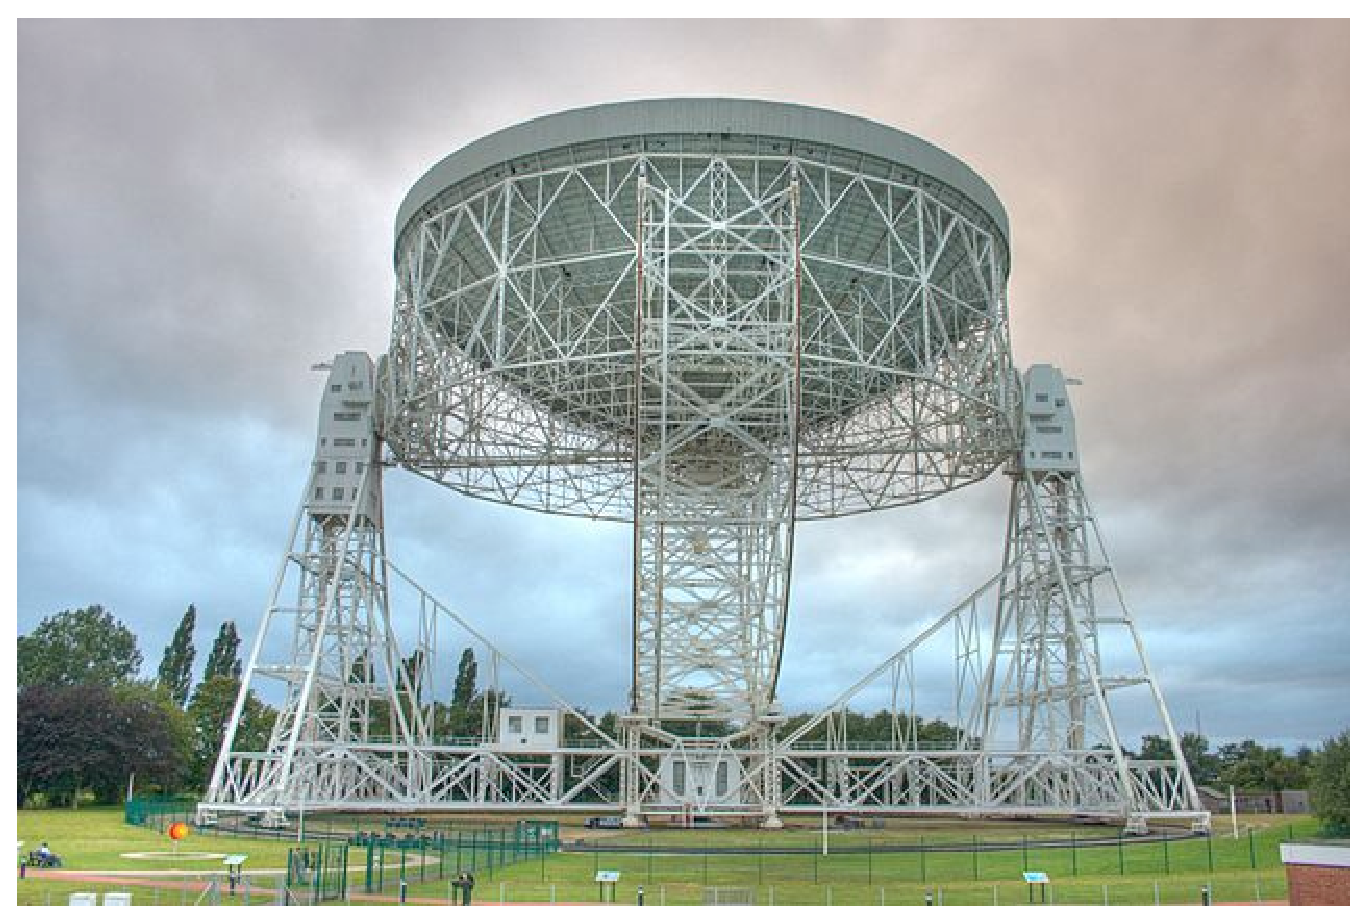
\includegraphics[scale=0.5]{Lovell_Telescope.eps}%
\caption{The Lovell Telescope, when constructed in 1955 it was the largest steerable dish radio telescope in the world.}
\end{center}\end{figure}

\begin{shaded}
\textbf{Exercise \theExercise \stepcounter{Exercise}} : Satellites transmitting television data, such as Freesat and Sky Digital in the UK, use radio signals in the K$_u$ band, these lie between 12 and 18 GHz. What are the wavelengths associated with these frequencies? Can satellite dishes used for television also be used for radio astronomy?\end{shaded}

Radio astronomy has a large drawback compared to visible-light astronomy, the wavelengths involved are much larger. This means that you need a far larger telescope (with a large parabolic mirror) to obtain a similar resolution. In the module `Telescopes' we explained how the resolution of a telescope can be determined.

Building one large telescope can be difficult. But the experience obtained during the use of the first telescopes offered a solution, it led to the development of radio interferometry. This technique uses multiple smaller telescopes placed on a line or a grid and combines the readings from all dishes to obtain one `image'.

Although one small satellite dish might not be enough for radio astronomy, three or four placed in line might be. All dishes need to be connected to the same monitoring station. Care must be taken in how this is done. Signals arriving at all dishes at the same time also need to arrive at the station at the same time. This means that the cables running from the dishes to the station all need to be of the same length. All other influences on the signal also need to be the same.

\begin{shaded}
\textbf{Exercise \theExercise \stepcounter{Exercise}} : Do a little on-line research. What do you need to build your own radio telescope? Can you build one your self? Are there amateur radio astronomers? What kind of (home made) setup do they use?\end{shaded}

\section{Resolution of a Radio Telescope}
According to the module `Telescopes' we can find the resolution of one telescope with:
\begin{equation}
\sin \alpha \approx \tan \alpha \approx \frac{\lambda}{\mbox{Diameter}} \label{eq:reso_sim}
\end{equation}
In this module with did not take diffraction into account. Because of diffraction a star (or other light source) will not appear as a single point in our image but will have airy disc around it. Because these airy discs are larger than the actual image of the star the resolution will be lower (the images start to overlap sooner). This means that equation~\ref{eq:reso_sim} should be modified into:
\begin{equation}
\sin \alpha \approx \tan \alpha \approx 1.220 \frac{\lambda}{\mbox{Diameter}} \label{eq:reso}
\end{equation}
They derivation of the factor 1.220 is beyond the scope of this text. 

If we are looking at microwaves with a wavelength of 2.5~cm using a dish 50~cm in diameter:
\begin{equation}
\sin \alpha \approx \tan \alpha \approx 1.220 \frac{2.5~\mbox{cm}}{50~\mbox{cm}}=0.061
\end{equation}
This means that the smallest angle we can distinguish is 3.5$^\circ$ or 0.061 radians.

What is the resolution of two telescopes combined? Take a look at figure~\ref{fig:line_setup}, here we have placed to telescopes on a line, both are looking in the same direction. A radio signal is coming straight towards the telescopes. The wave front is parallel to the line between the telescopes. This means that the signal arrives at the telescopes at the same time. The signal measured by the telescopes in synchronous, they measure the crest of the wave at exactly the same time.

What happens when the radio wave hits the telescopes at an angle? This is depicted in figure~\ref{fig:line_setup_angle}. If the angle is such that the wave arrives in the right telescope exactly one period before it arrives in the left telescopes the signals are once again synchronous (the difference in path length is exactly one wave length in this case). This means that this setup is equally sensitive for signals coming from this direction (and with this wave length) as it is for signals coming straight from above. 

\begin{figure}\begin{center}
\begin{picture}(0,0)%
\includegraphics{line_setup.eps}%
\end{picture}%
\setlength{\unitlength}{4144sp}%
%
\begingroup\makeatletter\ifx\SetFigFont\undefined%
\gdef\SetFigFont#1#2#3#4#5{%
  \reset@font\fontsize{#1}{#2pt}%
  \fontfamily{#3}\fontseries{#4}\fontshape{#5}%
  \selectfont}%
\fi\endgroup%
\begin{picture}(3534,1416)(79,-565)
\end{picture}%
\caption{An oblique incident radio wave.}\label{fig:line_setup}
\end{center}\end{figure}

\begin{figure}\begin{center}
\begin{picture}(0,0)%
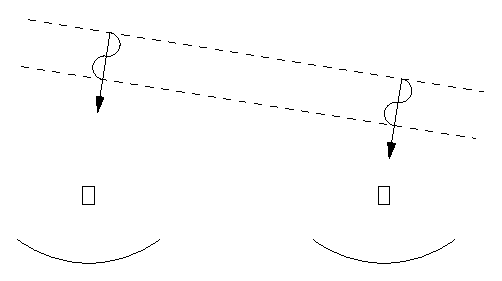
\includegraphics{line_setup_angle.eps}%
\end{picture}%
\setlength{\unitlength}{4144sp}%
%
\begingroup\makeatletter\ifx\SetFigFont\undefined%
\gdef\SetFigFont#1#2#3#4#5{%
  \reset@font\fontsize{#1}{#2pt}%
  \fontfamily{#3}\fontseries{#4}\fontshape{#5}%
  \selectfont}%
\fi\endgroup%
\begin{picture}(3568,1876)(173,-565)
\end{picture}%
\caption{Two telescopes placed on a line looking at the same object.}\label{fig:line_setup_angle}
\end{center}\end{figure}

\begin{shaded}
\textbf{Exercise \theExercise \stepcounter{Exercise}} : If you want a setup which is very sensitive for small angles, do you need to place the telescopes far apart or near to each other? Explain why.\end{shaded}
\begin{shaded}
\textbf{Exercise \theExercise \stepcounter{Exercise}} : If we were to place our telescopes very widely spaced, what would the effect be on the amount of synchronous signals?\end{shaded}
\begin{shaded}
\textbf{Exercise \theExercise \stepcounter{Exercise}} : If we want to look at only a very small fraction of the sky using three telescopes we need to place them on the corners of a (equilateral) triangle. Can you explain why?\end{shaded}

\section{Pulsars}
Dame (Susan) Jocelyn Bell Burnell worked together professor Hewish at Cambridge to build a radio telescope. The strength of the signals measured by the telescope were recorded on long strips of paper using an x,t-recorder (see figure~\ref{fig:recorder}). The setup was used to discover the presence of LGM, Little Green Men, extraterrestrial life. Unfortunately, the recorder wrote down data much faster than Bell could analyse them. In the huge amounts of data she eventually found a signal which repeated periodically. Could this be the sign of LGM?

To the researchers this seemed very unlikely because the periodically signals were found in multiple sections of the universe. More and more of these periodical repeating signals were found. Their explanation: rotating stars. We now call them pulsars. These stars act like lighthouses. They emit streams of high energy particles and because of the regular rotation we see this as a periodically repeating signal.

\begin{figure}[h]\begin{center}
\includegraphics[scale=0.12]{recorder.eps}%
\caption{A simple two channel x,t-recorder. Two pens are pressed against the paper which is fed through underneath the pens.}\label{fig:recorder}
\end{center}\end{figure}

\section{Constructing your own Interferometer Telescope}
To build an interferometer telescope you need the following materials:
\begin{itemize}
\item One or more dishes
\item One Low Noise Block downconverter (LNB\footnote{An LNB acts like a super-heterodyne receiver for satellite signals. In an heterodyne receiver the incoming signal is multiplied with an intermediate frequency. The result is a mix of signals at different frequencies. Filters can be used to allow certain signals or frequencies, such as UHF (ultra high frequency) or VHF (very high frequency), to pass. These signals can be understood by a TV-set. }) for every dish
\item A satellite finder (satellite signal meter)
\item Coax cables and splitters (75~$\Omega$)
\end{itemize}

Mount the LNB to the dish. Use a coax cable to connect the satellite finder. Do not forget to close of any unused connectors with a terminator cap, without the terminator unwanted reflections of the signal might occur. Using this one dish setup you can look for radio sources. The strength of the signal can be read out on the satellite finder. With a single dish the Sun can clearly be `seen', finding the Moon is already a lot harder.

We can expand our single dish setup with a second dish. Using a cable splitter both dished can be connected to the same satellite finder. The type of LNBs used determines (amongst others) whether or not this results in a signal which can be understood by the finder. When this does work, the finder will measure the sum of the two signals. This will greatly improve the resolution. The signals however need to be in phase. This means that the length of cable running to both dishes and LNBs much be the same length. The signals we are looking at have a wavelength of 2.5~cm, therefore the lengths of the cables must be accurate to the millimetre. If the cables are different in length one signal will be shifted with respect to the other, the result is a slanted view from the dishes (compare this to figure~\ref{fig:line_setup_angle}).

Time delays and phase differences are very important in an array setup. The mixing of the signals inside the LNBs also introduces a phase shift. Therefore, use the same LNB or intermediate frequency source on all the signals if possible. 

The array of dished can be further expanded using a third or even fourth dish. 


\end{document}


\begin{shaded}
\textbf{Exercise \theExercise \stepcounter{Exercise}} : \end{shaded}

\footnotemark
\footnotetext{}
